\documentclass[tikz,border=2pt]{standalone}
\usepackage{pgfplots}
\pgfplotsset{compat=1.18}
\usetikzlibrary{intersections}
\usepgfplotslibrary{fillbetween}


\begin{document}
	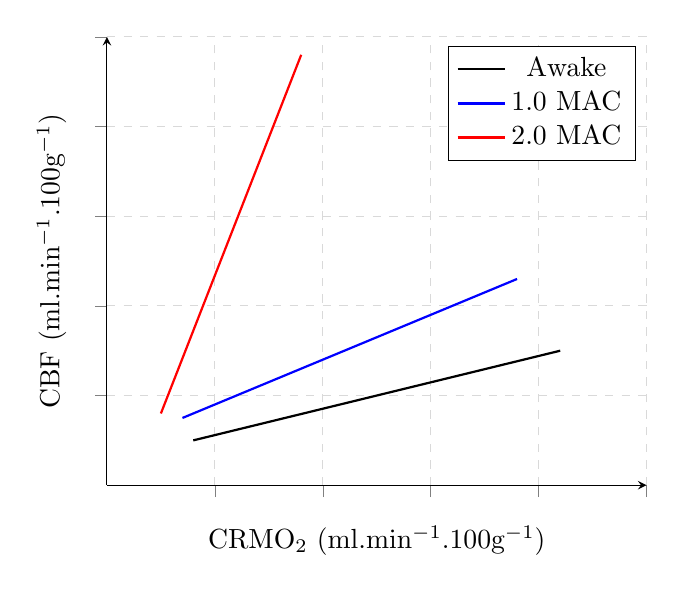
\begin{tikzpicture}
		\begin{axis}[
			axis lines=middle,
			ymin = 0,
			ymax = 5,
			xmin = 0,
			xmax= 5,
			grid = major,
			grid style={dashed, gray!30},
			ylabel near ticks,
			xlabel near ticks,
			xlabel= CRMO$_2$ (ml.min$^{-1}$.100g$^{-1}$),
			ylabel= CBF (ml.min$^{-1}$.100g$^{-1}$),
			tick align=outside,
			xticklabels={,,},
			yticklabels={,,}
			legend style={font=\small, cells={align=left}}]

			\draw [black, thick] (0.8,0.5) -- (4.2,1.5);
			\draw [blue, thick] (0.7,0.75) -- (3.8,2.3);
			\draw [red, thick] (0.5,0.8) -- (1.8,4.8);

		\addlegendimage{black, thick};
		\addlegendentry{Awake};
		\addlegendimage{blue, thick};
		\addlegendentry{1.0 MAC};
		\addlegendimage{red, thick};
		\addlegendentry{2.0 MAC};


		\end{axis}
	\end{tikzpicture} 
\end{document}